% Copyright (c) 2013, Christian Gehring, Hannes Sommer, Paul Furgale, Remo Diethelm
% All rights reserved.
%
% Redistribution and use in source and binary forms, with or without
% modification, are permitted provided that the following conditions are met:
%     * Redistributions of source code must retain the above copyright
%       notice, this list of conditions and the following disclaimer.
%     * Redistributions in binary form must reproduce the above copyright
%       notice, this list of conditions and the following disclaimer in the
%       documentation and/or other materials provided with the distribution.
%     * Neither the name of the Autonomous Systems Lab, ETH Zurich nor the
%       names of its contributors may be used to endorse or promote products
%       derived from this software without specific prior written permission.
%
% THIS SOFTWARE IS PROVIDED BY THE COPYRIGHT HOLDERS AND CONTRIBUTORS "AS IS" AND
% ANY EXPRESS OR IMPLIED WARRANTIES, INCLUDING, BUT NOT LIMITED TO, THE IMPLIED
% WARRANTIES OF MERCHANTABILITY AND FITNESS FOR A PARTICULAR PURPOSE ARE
% DISCLAIMED. IN NO EVENT SHALL Christian Gehring, Hannes Sommer, Paul Furgale,
% Remo Diethelm BE LIABLE FOR ANY DIRECT, INDIRECT, INCIDENTAL, SPECIAL, EXEMPLARY,
% OR CONSEQUENTIAL DAMAGES (INCLUDING, BUT NOT LIMITED TO, PROCUREMENT OF SUBSTITUTE
% GOODS OR SERVICES; LOSS OF USE, DATA, OR PROFITS; OR BUSINESS INTERRUPTION)
% HOWEVER CAUSED AND ON ANY THEORY OF LIABILITY, WHETHER IN CONTRACT, STRICT LIABILITY,
% OR TORT (INCLUDING NEGLIGENCE OR OTHERWISE) ARISING IN ANY WAY OUT OF THE USE OF THIS
% SOFTWARE, EVEN IF ADVISED OF THE POSSIBILITY OF SUCH DAMAGE.

\documentclass[10pt,landscape,a4paper]{article}
\usepackage{nonfloat}
\usepackage{multicol}
\usepackage[font=scriptsize]{caption}
\usepackage{calc}
\usepackage{ifthen}
\usepackage[landscape]{geometry}
\usepackage{amsmath}
\usepackage{amssymb}
\usepackage{multirow}
 \usepackage[T1]{fontenc}
% \usepackage{bbold}
    \usepackage{dsfont}
%\usepackage{esvect}
\usepackage{graphics}
   \usepackage[pdftex]{graphicx}

\usepackage{tabularx,booktabs} 
\usepackage{epstopdf}
 \usepackage{ifpdf}
\usepackage{sectsty}
\usepackage{tikz}
\usepackage{mathtools} % \mathclap for underbrace
\paragraphfont{\small}

% To make this come out properly in landscape mode, do one of the following
% 1.
%  pdflatex latexsheet.tex
%
% 2.
%  latex latexsheet.tex
%  dvips -P pdf  -t landscape latexsheet.dvi
%  ps2pdf latexsheet.ps


% If you're reading this, be prepared for confusion.  Making this was
% a learning experience for me, and it shows.  Much of the placement
% was hacked in; if you make it better, let me know...


% 2008-04
% Changed page margin code to use the geometry package. Also added code for
% conditional page margins, depending on paper size. Thanks to Uwe Ziegenhagen
% for the suggestions.

% 2006-08
% Made changes based on suggestions from Gene Cooperman. <gene at ccs.neu.edu>


% To Do:
% \listoffigures \listoftables
% \setcounter{secnumdepth}{0}


% This sets page margins to .5 inch if using letter paper, and to 1cm
% if using A4 paper. (This probably isn't strictly necessary.)
% If using another size paper, use default 1cm margins.
\ifthenelse{\lengthtest { \paperwidth = 11in}}
	{ \geometry{top=.5in,left=.5in,right=.5in,bottom=.5in} }
	{\ifthenelse{ \lengthtest{ \paperwidth = 297mm}}
		{\geometry{top=1cm,left=1cm,right=1cm,bottom=1cm} }
		{\geometry{top=1cm,left=1cm,right=1cm,bottom=1cm} }
	}

% Turn off header and footer
\pagestyle{empty}
 

% Redefine section commands to use less space
\makeatletter
\renewcommand{\section}{\@startsection{section}{1}{0mm}%
                                {-1ex plus -.5ex minus -.2ex}%
                                {0.5ex plus .2ex}%x
                                {\normalfont\large\bfseries}}
\renewcommand{\subsection}{\@startsection{subsection}{2}{0mm}%
                                {-1explus -.5ex minus -.2ex}%
                                {0.5ex plus .2ex}%
                                {\normalfont\normalsize\bfseries}}
\renewcommand{\subsubsection}{\@startsection{subsubsection}{3}{0mm}%
                                {-1ex plus -.5ex minus -.2ex}%
                                {1ex plus .2ex}%
                                {\normalfont\small\bfseries}}
\makeatother

% Define BibTeX command
\def\BibTeX{{\rm B\kern-.05em{\sc i\kern-.025em b}\kern-.08em
    T\kern-.1667em\lower.7ex\hbox{E}\kern-.125emX}}

% Don't print section numbers
\setcounter{secnumdepth}{0}


\setlength{\parindent}{0pt}
\setlength{\parskip}{0pt plus 0.5ex}


 % figures
\newcommand{\sizes}{3.4} % selbstdefinierte Punktgrösse in Bilder
\newcommand{\sizem}{5.1}% selbstdefinierte Punktgrösse in Bilder

%math
\newcommand{\dd}{\textnormal{d}}
\newcommand{\dt}{\textnormal{d}t}
\newcommand{\DD}{\textnormal{D}}
\newcommand{\Dt}{\textnormal{D}t}
\newcommand{\deta}{\textnormal{d}\eta}
\newcommand{\argmin}{\mathop{\mathrm{argmin}}}
\newcommand{\Upr}{{\mathop{\mathrm{Upr}}}}
\newcommand{\Sgn}{{\mathop{\mathrm{Sgn}}}}
\newcommand{\h}{\mathop{\mathrm{H}}}
\newcommand{\prox}{{\mathop{\mathrm{prox}}}}
\newcommand{\abs}{\mathop{\mathrm{abs}}}
\newcommand{\T}{^{\mathop{\mathrm{T}}}}
\newcommand{\diag}{{\mathop{\mathrm{diag}}}}


%boldmath
%bold operator
\newcommand{\vna}{\mbox{\boldmath $\nabla$}}
%bold greek
\newcommand{\val}{\mbox{\boldmath $\alpha$}}
\newcommand{\vbe}{\mbox{\boldmath $\beta$}}
\newcommand{\vga}{\mbox{\boldmath $\gamma$}}
\newcommand{\vde}{\mbox{\boldmath $\delta$}}
\newcommand{\vep}{\mbox{\boldmath $\epsilon$}}
\newcommand{\vze}{\mbox{\boldmath $\zeta$}}
\newcommand{\vet}{\mbox{\boldmath $\eta$}}
\newcommand{\vth}{\mbox{\boldmath $\theta$}}
\newcommand{\vio}{\mbox{\boldmath $\iota$}}
\newcommand{\vka}{\mbox{\boldmath $\kappa$}}
\newcommand{\vla}{\mbox{\boldmath $\lambda$}}
\newcommand{\vmu}{\mbox{\boldmath $\mu$}}
\newcommand{\vnu}{\mbox{\boldmath $\nu$}}
\newcommand{\vxi}{\mbox{\boldmath $\xi$}}
\newcommand{\vpi}{\mbox{\boldmath $\pi$}}
\newcommand{\vrh}{\mbox{\boldmath $\rho$}}
\newcommand{\vsi}{\mbox{\boldmath $\sigma$}}
\newcommand{\vta}{\mbox{\boldmath $\tau$}}
\newcommand{\vup}{\mbox{\boldmath $\upsilon$}}
\newcommand{\vph}{\mbox{\boldmath $\varphi$}}
\newcommand{\vch}{\mbox{\boldmath $\chi$}}
\newcommand{\vps}{\mbox{\boldmath $\psi$}}
\newcommand{\vom}{\mbox{\boldmath $\omega$}}

\newcommand{\vvep}{\mbox{\boldmath $\varepsilon$}}
\newcommand{\vvth}{\mbox{\boldmath $\vartheta$}}
\newcommand{\vvrh}{\mbox{\boldmath $\varrho$}}
\newcommand{\vvpi}{\mbox{\boldmath $\varpi$}}
\newcommand{\vvsi}{\mbox{\boldmath $\varsigma$}}
\newcommand{\vvph}{\mbox{\boldmath $\phi$}}

%bold capital greek
\newcommand{\vGa}{\mathbf \Gamma}
\newcommand{\vDe}{\mathbf \Delta}
\newcommand{\vTh}{\mathbf \Theta}
\newcommand{\vLa}{\mathbf \Lambda}
\newcommand{\vXi}{\mathbf \Xi}
\newcommand{\vPi}{\mathbf \Pi}
\newcommand{\vSi}{\mathbf \Sigma}
\newcommand{\vUp}{\mathbf \Upsilon}
\newcommand{\vPh}{\mathbf \Phi}
\newcommand{\vPs}{\mathbf \Psi}
\newcommand{\vOm}{\mathbf \Omega}

%capital greek slanted, OHNE amsmath-package
%\newcommand{\iGa}{\mathnormal{\Gamma}}
%\newcommand{\iDe}{\mathnormal{\Delta}}
%\newcommand{\iTh}{\mathnormal{\Theta}}
%\newcommand{\iLa}{\mathnormal{\Lambda}}
%\newcommand{\iXi}{\mathnormal{\Xi}}
%\newcommand{\iPi}{\mathnormal{\Pi}}
%\newcommand{\iSi}{\mathnormal{\Sigma}}
%\newcommand{\iUp}{\mathnormal{\Upsilon}}
%\newcommand{\iPh}{\mathnormal{\Phi}}
%\newcommand{\iPs}{\mathnormal{\Psi}}
%\newcommand{\iOm}{\mathnormal{\Omega}}

%capital greek slanted, MIT amsmath-package
\newcommand{\iGa}{\varGamma}
\newcommand{\iDe}{\varDelta}
\newcommand{\iTh}{\varTheta}
\newcommand{\iLa}{\varLambda}
\newcommand{\iXi}{\varXi}
\newcommand{\iPi}{\varPi}
\newcommand{\iSi}{\varSigma}
\newcommand{\iUp}{\varUpsilon}
\newcommand{\iPh}{\varPhi}
\newcommand{\iPs}{\varPsi}
\newcommand{\iOm}{\varOmega}

%bold latin
\newcommand{\va}{\mathbf a}
\newcommand{\vb}{\mathbf b}
\newcommand{\vc}{\mathbf c}
\newcommand{\vd}{\mathbf d}
\newcommand{\ve}{\mathbf e}
\newcommand{\vf}{\mathbf f}
\newcommand{\vg}{\mathbf g}
\newcommand{\vh}{\mathbf h}
\newcommand{\vi}{\mathbf i}
\newcommand{\vj}{\mathbf j}
\newcommand{\vk}{\mathbf k}
\newcommand{\vl}{\mathbf l}
\newcommand{\vm}{\mathbf m}
\newcommand{\vn}{\mathbf n}
\newcommand{\vo}{\mathbf o}
\newcommand{\vp}{\mathbf p}
\newcommand{\vq}{\mathbf q}
\newcommand{\vr}{\mathbf r}
\newcommand{\vs}{\mathbf s}
\newcommand{\vt}{\mathbf t}
\newcommand{\vu}{\mathbf u}
\newcommand{\vv}{\mathbf v}
\newcommand{\vw}{\mathbf w}
\newcommand{\vx}{\mathbf x}
\newcommand{\vy}{\mathbf y}
\newcommand{\vz}{\mathbf z}
\newcommand{\eins}{\mathbf 1}

%bold capital latin
\newcommand{\vA}{\mathbf A}
\newcommand{\vB}{\mathbf B}
\newcommand{\vC}{\mathbf C}
\newcommand{\vD}{\mathbf D}
\newcommand{\vE}{\mathbf E}
\newcommand{\vF}{\mathbf F}
\newcommand{\vG}{\mathbf G}
\newcommand{\vH}{\mathbf H}
\newcommand{\vI}{\mathbf I}
\newcommand{\vJ}{\mathbf J}
\newcommand{\vK}{\mathbf K}
\newcommand{\vL}{\mathbf L}
\newcommand{\vM}{\mathbf M}
\newcommand{\vN}{\mathbf N}
\newcommand{\vO}{\mathbf O}
\newcommand{\vP}{\mathbf P}
\newcommand{\vQ}{\mathbf Q}
\newcommand{\vR}{\mathbf R}
\newcommand{\vS}{\mathbf S}
\newcommand{\vT}{\mathbf T}
\newcommand{\vU}{\mathbf U}
\newcommand{\vV}{\mathbf V}
\newcommand{\vW}{\mathbf W}
\newcommand{\vX}{\mathbf X}
\newcommand{\vY}{\mathbf Y}
\newcommand{\vZ}{\mathbf Z}

%calligraphic
\newcommand{\cA}{\mathcal{A}}
\newcommand{\cB}{\mathcal{B}}
\newcommand{\cC}{\mathcal{C}}
\newcommand{\cD}{\mathcal{D}}
\newcommand{\cE}{\mathcal{E}}
\newcommand{\cF}{\mathcal{F}}
\newcommand{\cG}{\mathcal{G}}
\newcommand{\cH}{\mathcal{H}}
\newcommand{\cI}{\mathcal{I}}
\newcommand{\cJ}{\mathcal{J}}
\newcommand{\cK}{\mathcal{K}}
\newcommand{\cL}{\mathcal{L}}
\newcommand{\cM}{\mathcal{M}}
\newcommand{\cN}{\mathcal{N}}
\newcommand{\cO}{\mathcal{O}}
\newcommand{\cP}{\mathcal{P}}
\newcommand{\cQ}{\mathcal{Q}}
\newcommand{\cR}{\mathcal{R}}
\newcommand{\cS}{\mathcal{S}}
\newcommand{\cT}{\mathcal{T}}
\newcommand{\cU}{\mathcal{U}}
\newcommand{\cV}{\mathcal{V}}
\newcommand{\cW}{\mathcal{W}}
\newcommand{\cX}{\mathcal{X}}
\newcommand{\cY}{\mathcal{Y}}
\newcommand{\cZ}{\mathcal{Z}}

%fraktur
\newcommand{\frA}{\mathfrak{A}}
\newcommand{\frB}{\mathfrak{B}}
\newcommand{\frC}{\mathfrak{C}}
\newcommand{\frD}{\mathfrak{D}}
\newcommand{\frE}{\mathfrak{E}}
\newcommand{\frF}{\mathfrak{F}}
\newcommand{\frG}{\mathfrak{G}}
\newcommand{\frH}{\mathfrak{H}}
\newcommand{\frI}{\mathfrak{I}}
\newcommand{\frJ}{\mathfrak{J}}
\newcommand{\frK}{\mathfrak{K}}
\newcommand{\frL}{\mathfrak{L}}
\newcommand{\frM}{\mathfrak{M}}
\newcommand{\frN}{\mathfrak{N}}
\newcommand{\frO}{\mathfrak{O}}
\newcommand{\frP}{\mathfrak{P}}
\newcommand{\frQ}{\mathfrak{Q}}
\newcommand{\frR}{\mathfrak{R}}
\newcommand{\frS}{\mathfrak{S}}
\newcommand{\frT}{\mathfrak{T}}
\newcommand{\frU}{\mathfrak{U}}
\newcommand{\frV}{\mathfrak{V}}
\newcommand{\frW}{\mathfrak{W}}
\newcommand{\frX}{\mathfrak{X}}
\newcommand{\frY}{\mathfrak{Y}}
\newcommand{\frZ}{\mathfrak{Z}}

\newcommand{\fra}{\mathfrak{a}}
\newcommand{\frb}{\mathfrak{b}}
\newcommand{\frc}{\mathfrak{c}}
\newcommand{\frd}{\mathfrak{d}}
\newcommand{\fre}{\mathfrak{e}}
\newcommand{\frf}{\mathfrak{f}}
\newcommand{\frg}{\mathfrak{g}}
\newcommand{\frh}{\mathfrak{h}}
\newcommand{\fri}{\mathfrak{i}}
\newcommand{\frj}{\mathfrak{j}}
\newcommand{\frk}{\mathfrak{k}}
\newcommand{\frl}{\mathfrak{l}}
\newcommand{\frm}{\mathfrak{m}}
\newcommand{\frn}{\mathfrak{n}}
\newcommand{\fro}{\mathfrak{o}}
\newcommand{\frp}{\mathfrak{p}}
\newcommand{\frq}{\mathfrak{q}}
\newcommand{\frr}{\mathfrak{r}}
\newcommand{\frs}{\mathfrak{s}}
\newcommand{\frt}{\mathfrak{t}}
\newcommand{\fru}{\mathfrak{u}}
\newcommand{\frv}{\mathfrak{v}}
\newcommand{\frw}{\mathfrak{w}}
\newcommand{\frx}{\mathfrak{x}}
\newcommand{\fry}{\mathfrak{y}}
\newcommand{\frz}{\mathfrak{z}}

% -----------------------------------------------------------------------
\DeclareGraphicsExtensions{.pdf,.eps}

 \DeclareMathOperator{\tr}{tr}
 \DeclareMathOperator{\logmap}{log}
 \DeclareMathOperator{\expmap}{exp}
 \DeclareMathOperator{\logmatrix}{logM}
 \DeclareMathOperator{\expmatrix}{expM}
% identity matrix
\newcommand\identity{\mathds{1}}
\newcommand\zero{\mathbf{0}}
\newcommand\norm[1]{\lVert #1 \rVert}
\newcommand\transpose{\mathsf{T}}

\newcommand\imquatvec[1]{\overrightarrow{\mathbf{#1}}}

\newcommand\pos[3]{{}_#1\vr_{#2\!#3}}
\newcommand\postranspose[3]{{}_#1\vr_{#2\!#3}^\transpose}
\newcommand\rotmat[2]{\vR_{#1\!#2}}
\newcommand\drotmat[2]{\dot{\vR}_{#1\!#2}}
\newcommand\comat[2]{\vC_{#1\!#2}}
\newcommand\dcomat[2]{\dot{\vC}_{#1\!#2}}
\newcommand\quat[2]{\vp_{#1\!#2}}
\newcommand\Quat[2]{P_{#1\!#2}}
\newcommand\angleaxis[2]{(\theta,\vn)_{#1\!#2}}
\newcommand\rotvec[2]{\vvph_{#1\!#2}}
\newcommand\linvel[2]{{}_#1\vv_{#2}}
\newcommand\rotvel[3]{{}_#1\vom_{#2\!#3}}
\newcommand\rotvelhat[3]{{}_#1\hat{\vom}_{#2\!#3}}

\newcommand\myfigure[1]{%
\medskip\noindent\begin{minipage}{\columnwidth}
\centering%
#1%
%figure,caption, and label go here
\end{minipage}\medskip}

\begin{document}

\raggedright
\footnotesize
\begin{multicols}{2}


% multicol parameters
% These lengths are set only within the two main columns
%\setlength{\columnseprule}{0.25pt}
\setlength{\premulticols}{1pt}
\setlength{\postmulticols}{1pt}
\setlength{\multicolsep}{1pt}
\setlength{\columnsep}{2pt}

\begin{center}
     \Large{\textbf{Kindr Cheat Sheet}} \\
      \small{Kinematics and Dynamics for Robotics}
\end{center}
%%%%%%%%%%%%%%%%%%%%%%%%%%%%%%%%%%%%%%%%%%%%%%%%%%%%%%%%%%%%%%%%%%%%%%%%%%%%%%%%%%%%%%%
%  BEGIN CONTENT
%%%%%%%%%%%%%%%%%%%%%%%%%%%%%%%%%%%%%%%%%%%%%%%%%%%%%%%%%%%%%%%%%%%%%%%%%%%%%%%%%%%%%%%
\section{Nomenclature }
\begin{tabular}{|l|l@{}|l|}
\hline
(Hyper-)complex number & $Q$ & normal capital letter  \\ \hline
Column vector & $\va$ & bold small letter  \\ \hline
Matrix & $\vM$ & bold capital letter  \\ \hline
Identity matrix & $\identity_{n\times m}$ & ${n \times m}$-matrix  \\  \hline
Coordinate system (CS) & ${\ve_x^A,\ve_y^A,\ve_z^A}$ & Cartesian right-hand system $A$ with basis (unit) vectors $\ve$  \\ \hline
Inertial frame & ${\ve_x^I,\ve_y^I,\ve_z^I}$ & Global / inertial / world coordinate system (never moves) \\ \hline
Body-fixed frame & ${\ve_x^B,\ve_y^B,\ve_z^B}$ & Local / body-fixed coordinate system (moves with body) \\ \hline
Rotation & $\cR \in \mathrm{SO}(3)$ & generic rotation (for all parameterizations) \\ \hline
Machine precision & $\epsilon$ & \\ \hline
%Translational velocity & $\linvel{I}{P} \in \mathbb{R}^3 $  & translational velocity of point $P$ expressed in CS $I$ \\ \hline
%Angular velocity & $\rotvel{I}{I}{B} \in \mathbb{R}^3 $ & ang. velocity of CS $B$ w.r.t. to CS $B$ expressed in CS $I$ \\ \hline
%Ang. vel. of rigid body & ${}_B\vOm = \rotvel{B}{I}{B}$ & with body-fixed CS $B$ and inertial CS $I$ \\ \hline
%Ang. acc. of rigid body & ${}_B\vPs$ \\ \hline

% Generalized coordinates & $\vq \in \mathbb{Q} \subset \mathbb{R}^{n_q}$ & set of coordinates to describe a multi-rigid-body system\\ \hline
% Generalized velocities & $\vu \in \mathbb{U} \subset \mathbb{R}^{n_u}$ & gen. velocities of multi-rigid-body system, where $\vu = \vF\dot{\vq}$\\ \hline
\end{tabular}
\section{Operators}
\begin{tabular}{|l|l|}
\hline
Cross product & $\va \times \vb = \begin{bmatrix} a_1 \\ a_2 \\ a_3\end{bmatrix} \times \begin{bmatrix} b_1 \\ b_2 \\ b_3\end{bmatrix} \Leftrightarrow (\va)^\wedge \vb = \hat{\va}\vb = \begin{bmatrix} 0 & -a_3 & a_2 \\ a_3 & 0 & -a_1 \\ -a_2 & a_1 & 0 \end{bmatrix} \begin{bmatrix} b_1 \\ b_2 \\ b_3\end{bmatrix}$ \\ \hline
Skew/unskew &  $ \va = \hat{\va}^\vee$ \\ \hline
Euclidean norm & $\norm{\va} = \sqrt{\va^T\va} = \sqrt{a_1^2 + \ldots + a_n^2}$ \\ \hline
Exponential map for matrix & $\expmatrix: \mathbb{R}^3 \rightarrow \mathbb{R}^3,  \vA \mapsto e^\vA, \quad \vA \in \mathbb{R}^{3\times 3}$ \\ \hline
Logarithmic map for matrix & $\logmatrix: \mathbb{R}^3 \rightarrow \mathbb{R}^3, \vA \mapsto \log{\vA}, \quad  \vA \in \mathbb{R}^{3\times 3}$\\ \hline
\end{tabular}

\section{Position \& Orientation}
\subsection{Position}
\begin{tabular}{|l|l|l|}
 \hline
Vector & $\vr_{O\!P}$ & from point $O$ to point $P$ \\ \hline
Position vector & $\pos{A}{O}{P} \in \mathbb{R}^3 $ & from point $O$ to point $P$ expr. in frame $A$ \\ \hline 
Homogeneous pos. vector & ${}_A\bar{\vr}_{O\!P} = \begin{bmatrix}\postranspose{A}{O}{P} & 1 \end{bmatrix}^\transpose$ & from point $O$ to point $P$ expr. in frame $A$ \\ \hline
\end{tabular}


\subsection{Orientation/Rotation}
\parbox[t]{0.7\columnwidth}{\null
  \vskip-\abovecaptionskip
\begin{tabular}[h!]{r@{ }p{3cm}@{ }l@{ }}
 1) & Active Rotation: & $\cR^A: {}_A\color{blue}{\vr_{O\!P}} \color{black}\mapsto {}_A\color{green!50!black}{\vr_{O\!Q}} $ (rotates the vector $\vr_{O\!P}$) \\
 2) & Passive Rotation:& $\cR^P: {}_A\color{blue}{\vr_{O\!P}} \color{black}\mapsto \color{red}{}_B\color{blue}{\vr_{O\!P}} $ (rotates the frame $(\ve_x^A,\ve_y^A,\ve_z^A)$)\\
 3) & Inversion: & $\cR^{A^{-1}}(\vr) = \cR^P(\vr)$ \\ 
 4) & Concatenation: & \multicolumn{1}{l}{$\begin{aligned}\cR_2^A\left(\cR_1^A(\vr)\right) &= \left(\cR_2^A \otimes \cR_1^A\right)(\vr) \\ 
											    &= \left(\cR_1^{A^{-1}} \otimes \cR_2^{A^{-1}}\right)^{-1}(\vr) \\
                                            \cR_2^P\left(\cR_1^P(\vr)\right) &= \left(\cR_2^P \otimes \cR_1^P\right)(\vr) \\ 
									     &= \left(\cR_1^{P^{-1}} \otimes \cR_2^{P^{-1}}\right)^{-1}(\vr) \\
					      \end{aligned}$} \\
 5) & Exponential map: & $ \expmap: \mathbb{R}^3 \rightarrow \mathrm{SO}(3), \vv \mapsto \expmatrix(\hat{\vv}), \quad \vv \in \mathbb{R}^3$ \\
 6) & Logarithmic map: & $ \logmap: \mathrm{SO}(3) \rightarrow \mathbb{R}^3, \cR \mapsto \logmatrix(\cR)^\vee, \quad \cR \in \mathrm{SO}(3)$ \\ 
 7) & Box plus: & $\cR_{2} = \cR_{1} \boxplus \vv = \expmap{(\vv)} \otimes \cR_{1}, \quad  \cR_1, \cR_2 \in \mathrm{SO}(3), \vv \in \mathbb{R}^3$   \\
 8) & Box minus: & $\vv = \cR_{1} \boxminus \cR_2 = \logmap{(\cR_1\otimes\cR_2^{-1})}, \quad \cR_1, \cR_2 \in \mathrm{SO}(3), \vv \in \mathbb{R}^3$  \\ 
 9) & Discrete integration: & $\cR^{k+1} = \cR^k \boxplus ({}_B\vom_{I\!B}\Delta t)$ \\
 10) & (Spherical) linear interpolation $t \in [0, 1]$: & $\begin{aligned}\cR_t &= \cR_0 \boxplus \left( (\cR_1 \boxminus \cR_0) t \right), \quad \cR_t = \cR(t), \cR_0 = \cR(0), \cR_1=\cR(1) \\ &= (\cR_1 \otimes \cR_0^{-1})^t \otimes \cR_0 \end{aligned}$ \\ 
\end{tabular}
}
\parbox[t]{0.25\columnwidth}{\null
\vspace{-5mm}
        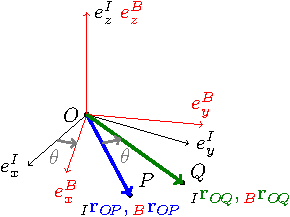
\includegraphics[width=0.25\columnwidth]{coordinate_systems/rotation_active_passive-crop.pdf}
}

\begin{tabular}{|l|l@{}|l@{}|}
\hline
%Rotation Matrix &  $\rotmat{B}{A}  =\begin{bmatrix} R_{11} & R_{12} & R_{13} \\  R_{21} & R_{22} & R_{23} \\ R_{31} & R_{32} & R_{33} \end{bmatrix} \in \mathrm{SO}(3)$ & Maps the coord. of the basis vectors $(_A\ve_x^A, _A\ve_y^A, _A\ve_z^A)$ \\
Rotation Matrix &  $\rotmat{B}{A} \in \mathrm{SO}(3)$ & Maps the coord. of the basis vectors $(_A\ve_x^A, _A\ve_y^A, _A\ve_z^A)$ \\
 & $ \pos{A}{O}{Q} = \rotmat{B}{A} \pos{A}{O}{P}$ & of frame $A$ expressed in $A$  into the coordinates of the  \\
& $ \pos{B}{O}{P} = \rotmat{B}{A}^\transpose \pos{A}{O}{P}$ & basis vectors $(_A\ve_x^B, _A\ve_y^B, _A\ve_z^B)$ of $B$ expressed in $A$. \\ 
 & &  The rotation is active (alibi). \\
& & $_A\rotmat{B}{A} = \begin{bmatrix}_A\ve_x^B & _A\ve_y^B & _A\ve_z^B\end{bmatrix}$ \\ \hline
Direct Cosine& $\comat{B}{A} \in \mathrm{SO}(3)$ & The coordinate tranformation matrix, which transforms \\  
 Matrix & $ \pos{B}{O}{P} = \comat{B}{A} \pos{A}{O}{P}$ & vectors from frame $A$ to frame $B$. \\
& $\comat{B}{A} = \rotmat{B}{A}^\transpose$ & The rotation is passive (alias). \\  \hline 
 Rotation  & $\quat{B}{A}$ & The rotation is active (alibi). \\
Quaternion &   $\quat{B}{A} \Leftrightarrow \rotmat{B}{A} $ &  \\ \hline
Rotation & $\angleaxis{B}{A}$ &   Rotation with unit rotation axis $\vn$ and angle $\theta \in [0, \pi]$. \\
Angle-axis & $\angleaxis{B}{A} \Leftrightarrow \rotmat{B}{A}$  & The rotation is active (alibi). \\ \hline
Rotation Vector & $ \rotvec{B}{A} $  &  Rotation with rotation axis $\vn = \frac{\vvph}{\norm{\vvph}}$ and angle $\theta = \norm{\vvph}$. \\ 
 & $\rotvec{B}{A} \Leftrightarrow \rotmat{B}{A} $ &  The rotation is active (alibi). \\ \hline
Euler Angles ZYX &  $(\psi, \theta, \phi)_{B\!A}$  & Tait-Bryan angles (Flight conv.): $z-y'-x''$, i.e.\   \\
Euler Angles YPR & $(\psi, \theta, \phi)_{B\!A} \Leftrightarrow \comat{B}{A} $ & yaw-pitch-roll. Singularities are at $\theta=\pm\frac{\pi}{2}$. \\
 &  & $\psi\in[-\pi,\pi), \theta\in[-\frac{\pi}{2},\frac{\pi}{2}), \phi\in[-\pi,\pi)$  \\  \hline
Euler Angles XYZ &  $(\alpha, \beta, \gamma)_{B\!A}$ & Cardan angles (Glocker conv.): $x-y'-z''$, i.e.\ \\
Euler Angles RPY & $(\alpha, \beta, \gamma)_{B\!A} \Leftrightarrow \comat{B}{A}$ & roll-pitch-yaw. Singularities are at $\beta=\pm\frac{\pi}{2}$.  \\
 &  & $\alpha\in[-\pi,\pi), \beta\in[-\frac{\pi}{2},\frac{\pi}{2}), \gamma\in[-\pi,\pi)$  \\  \hline
\end{tabular} % \multirow{2}{*}{}

\subsubsection{Rotation Quaternion}
A rotation quaternion is a Hamiltonian unit quaternion: \\
$\boxed{\begin{aligned}P &= p_0 + p_1 i + p_2 j + p_3 k \in \mathbb{H}, \quad p_i \in \mathbb{R} \\
i^2 &= j^2=k^2 = ijk = -1, \quad \norm{P}= \sqrt{p_0^2 + p_1^2 + p_2^2 + p_3^2} = 1 \\
\end{aligned}}$   \\
Note that $\Quat{B}{A}$ and $-\Quat{B}{A}$ represent the same rotation, but not the same unit quaternion. \\
Rot. quaternion as tuple: $P = (p_0, p_1, p_2, p_3) = (p_0, \imquatvec{p})$ with $\imquatvec{p} := (p_1, p_2, p_3)^\transpose $ \\
Rot. quaternion as vector: $\vp = \begin{bmatrix} p_0 & p_1 & p_2 & p_3 \end{bmatrix}^\transpose $\\
% Imaginary part: $\overrightarrow{\vp} := (p_1, p_2, p_3)^\transpose$
% Real part: $p_0 = \vP_\mathnormal{Re}\vp $ \\

% Imaginary part: $\vp_{1:3} := \vP_\mathnormal{Im}\vp = \begin{bmatrix} p_1 & p_2 & p_3 \end{bmatrix}^\transpose $\\

Conjugate: $P^\ast = (p_0, -\imquatvec{p})$ \\
Inverse: $P^{-1} = P^\ast = (p_0, -\imquatvec{p})$ \\
%  The Eq. 109 and Eq. 111 in J. Diebel, 'Representating Attitude: Euler Angles, Unit Quaternions, and Rostation Vectors', Standford University, 2006. are wrong, they should be switched.
Quaternion multiplication: $\begin{aligned}Q \cdot P &= (q_0, \imquatvec{q})\cdot(p_0, \imquatvec{p}) = (q_0 p_0 - \imquatvec{q}^\transpose \imquatvec{p}, q_{0} \imquatvec{p} + p_0 \imquatvec{q} + \imquatvec{q} \times \imquatvec{p}) \quad \Leftrightarrow \\
	   \vq \otimes \vp &= \underbrace{\vQ(\vq)}_{\mathclap{\text{quaternion matrix}}}\vp \, = \, \begin{pmatrix}q_0 & -\imquatvec{q}^\transpose \\  \imquatvec{q} & q_0\identity_{3 \times 3}+\hat{\imquatvec{q}} \\ \end{pmatrix} \begin{pmatrix} p_0 \\ p_1 \\ p_2 \\ p_3 \end{pmatrix} 
	  = \begin{pmatrix} 
 q_0 & -q_1 & -q_2 & -q_3 \\
 q_1 &  q_0 & -q_3 &  q_2 \\
 q_2 &  q_3 &  q_0 & -q_1 \\
 q_3 & -q_2 &  q_1 &  q_0 \\ \end{pmatrix}\begin{pmatrix} p_0 \\ p_1 \\ p_2 \\ p_3 \end{pmatrix} \\
 &= \underbrace{\bar{\vQ}(\vp)}_{\mathclap{\text{conjugate quat. matrix}}}\vq \, = \, \begin{pmatrix}p_0 & -\imquatvec{p}^\transpose \\  \imquatvec{p} & p_0\identity_{3 \times 3}-\hat{\imquatvec{p}} \\ \end{pmatrix} \begin{pmatrix} q_0 \\ q_1 \\ q_2 \\ q_3 \end{pmatrix} 
	  = \begin{pmatrix} 
 p_0 & -p_1 & -p_2 & -p_3 \\
 p_1 &  p_0 & p_3 &  -p_2 \\
 p_2 &  -p_3 &  p_0 & p_1 \\
 p_3 & p_2 &  -p_1 &  p_0 \\ \end{pmatrix}\begin{pmatrix} q_0 \\ q_1 \\ q_2 \\ q_3 \end{pmatrix} \\
\end{aligned}$ \\


%$\begin{aligned}{}_B\vr_{OP} &= {}_I\vr_{OP} + 2a_0\tilde{\va} {}_I\vr_{OP} + 2 \tilde{\va}^2 {}_I\vr_{OP}, \quad  \text{(Eigen)} \\
% &= \vp_{BI} (0, {}_I\vr_{OP}^T)^T \vp_{BI}^{-1} = (a_0, \va^T)^T (0, {}_I\vr_{OP}^T)^T (a_0, -\va^T)^T \end{aligned}$



\subsubsection{Rotation Quaternion $\Leftrightarrow$ Rotation Angle-Axis}

\begin{tabular}{@{}lll@{}} 
$ \quat{B}{I} = \begin{bmatrix} \cos{\frac{\theta}{2}} \\ \vn \sin{\frac{\theta}{2}} \end{bmatrix}$ & $\Leftrightarrow$ & $
(\theta, \vn)_{B\!I} = \left\{
  \begin{array}{l l}
    (2\arccos{(p_0)}, \frac{\imquatvec{p}}{\norm{\imquatvec{p}}}) & \quad \text{if $\lVert \imquatvec{p} \rVert^2 \geq \epsilon^2$}\\
    (0, \begin{bmatrix}1 & 0 & 0\end{bmatrix}^\transpose)  & \quad \text{otherwise}
  \end{array} \right. $ \\
\end{tabular}
\subsubsection{Rotation Quaternion $\Leftrightarrow$ Direction Cosine Matrix }
$\begin{aligned}\comat{A}{B} &= \rotmat{A}{B}^\transpose(\quat{A}{B}) =  \identity_{3\times 3} + 2 p_0\hat{\imquatvec{p}} + 2 \hat{\imquatvec{p}}^2    \\
&= \begin{bmatrix}
 p_0^2 + p_1^2 - p_2^2 - p_3^2 &         2p_1p_2 - 2p_0p_3 &         2p_0p_2 + 2p_1p_3 \\
         2p_0p_3 + 2p_1p_2 & p_0^2 - p_1^2 + p_2^2 - p_3^2 &         2p_2p_3 - 2p_0p_1 \\
         2p_1p_3 - 2p_0p_2 &         2p_0p_1 + 2p_2p_3 & p_0^2 - p_1^2 - p_2^2 + p_3^2 \\ \end{bmatrix} \\
\end{aligned}$
%= \begin{pmatrix} 1 - 2 a_2^2 - 2 a_3^2  &     2 a_1 a_2 - 2 a_0 a_3 &     2 a_0 a_2 + 2 a_1 a_3 \\
     %2 a_0 a_3 + 2 a_1 a_2 & 1 - 2 a_1^2 - 2 a_3^2 &     2 a_2 a_3 - 2 a_0 a_1 \\
     %2 a_1 a_3 - 2 a_0 a_2 &     2 a_0 a_1 + 2 a_2 a_3 & 1 - 2 a_1^2 - 2 a_2^2  \\
%\end{pmatrix}

$\begin{aligned}\comat{B}{A} &= \rotmat{B}{A}^\transpose =  \rotmat{A}{B}(\quat{A}{B}) = \identity_{3 \times 3} - 2 p_0\hat{\imquatvec{p}} + 2 \hat{\imquatvec{p}}^2 \\
&= \begin{bmatrix}  p_0^2 + p_1^2 - p_2^2 - p_3^2 &         2p_0p_3 + 2p_1p_2 &         2p_1p_3 - 2p_0p_2 \\
         2p_1p_2 - 2p_0p_3 & p_0^2 - p_1^2 + p_2^2 - p_3^2 &         2p_0p_1 + 2p_2p_3 \\
         2p_0p_2 + 2p_1p_3 &         2p_2p_3 - 2p_0p_1 & p_0^2 - p_1^2 - p_2^2 + p_3^2 \\ \end{bmatrix}  \\  
\end{aligned}$ \\

$\vp_{BA} = \vp_{BA}(\comat{A}{B}) = \begin{bmatrix} \frac{1}{2} \sqrt{1 + \tr(\vC)} \\ \frac{C_{32} - C_{23}}{4 p_0} \\ \frac{C_{13} - C_{31}}{4 p_0} \\ \frac{C_{21} - C_{12}}{4 p_0} \end{bmatrix} \quad \text{if $\tr{(\vC	)} > 0 $}$ ($\comat{A}{B} \rightarrow \quat{B}{A}$ is not unique)

\subsubsection{Euler Angles ZYX $\Leftrightarrow$ Direction Cosine Matrix}
\myfigure{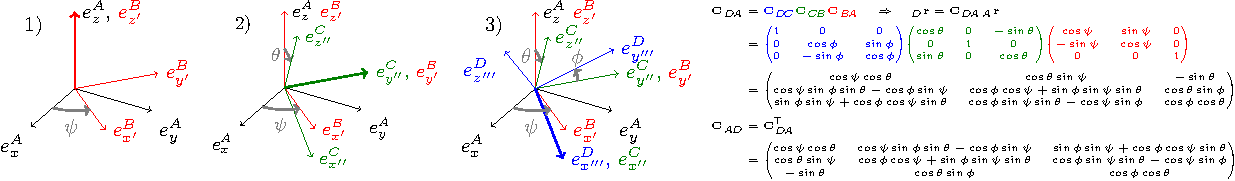
\includegraphics[width=1\columnwidth]{coordinate_systems/coordinate_system_ypr-crop.pdf}\vspace{-3mm}
\figcaption{Rotation from $I$-frame to $B$-frame: ($z-y'-x''$) -- (yaw-pitch-roll) -- ($\psi-\theta-\phi$) -- ($50^\circ-25^\circ-30^\circ)$}\label{fig:yaw-pitch-roll}}
\subsubsection{Euler Angles XYZ $\Leftrightarrow$ Direction Cosine Matrix}
\myfigure{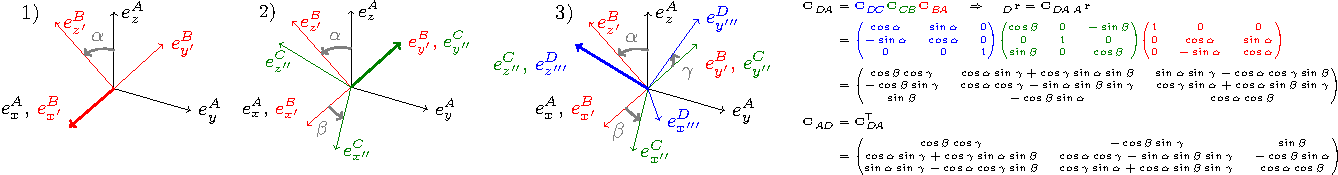
\includegraphics[width=1\columnwidth]{coordinate_systems/coordinate_system_rpy-crop.pdf}\vspace{-3mm}
\figcaption{Rotation from $I$-frame to $B$-frame: ($x-y'-z''$) -- (roll-pitch-yaw) -- ($\alpha-\beta-\gamma$) -- ($50^\circ-25^\circ-30^\circ)$}\label{fig:roll-pitch-yaw}}


% \subsection{Eigen Library}
% \begin{tabular}{@{}ll@{}} 
%  \verb!Vector3d ypr_BI = Vectord(psi,theta, phi);!  \\
%  \verb!aa_BI = AngleAxis(ypr_BI(0), Vector3d::UnitZ())*! \\
%  \verb!        AngleAxis(ypr_BI(1), Vector3d::UnitY())*! \\
%  \verb!        AngleAxis(ypr_BI(2), Vector3d::UnitX());! \\ 
%  \verb!Quaterniond p_BI = Quaterniond(aa_BI);! \\
%  \verb!Matrix3d A_IB = p_BI.toRotationMatrix();! \\
%  \verb!Vector3d I_r_OP = A_IB*B_r_OP! & \\
% \end{tabular}



% \subsubsection{Successive Composition of Rotations}
% $\vp_{IB} = \vp_{ID} \vp_{DC} \vp_{CB} \Leftrightarrow \vA_{BI} = \vA_{BC}\vA_{CD}\vA_{DI}$
% 
% \subsubsection{Transformation of a Vector}
% 
% ${}_{B}\vr_{OP} = \vA_{BI} {}_{I}\vr_{OP}$
% 
% $(0, {}_B\vr_{OP}) = \vp_{IB} (0, {}_I\vr_{OP}) \vp_{IB}^{-1}$ ????

\subsection{Pose}
\begin{tabular}{|l|l|l|}
\hline
Homogeneous Transformation Matrix & $\vT_{A\!B}$ &   \\ \hline
\end{tabular}

\subsubsection{Homogeneous Transformation Matrix}
 $\vT_{A\!B} = \begin{bmatrix}
              \comat{A}{B} & \pos{A}{A}{B} \\
	      \zero^\transpose & 1 \\
             \end{bmatrix}$

\section{Time Derivatives of Position \& Orientation}

\subsection{Linear Velocity}
Velocity of point $P$ expressed in frame $B$  w.r.t. to the inertial frame $I$: \\
${}_B\vv_P = {}_B\vv_A  + {}_B\dot{\vr}_{AP} + \rotvel{B}{I}{B} \times \pos{B}{A}{P}$ \\
Velocity of point $Q$ on rigid body $B$ that rotates with ${}_B\vOm$, where point $P$ is on the same rigid body $B$: \\
${}_B\vv_Q = {}_B\vv_{P} + {}_B\vOm \times \pos{B}{P}{Q}, \quad {}_B\vOm=\rotvel{B}{I}{B}$ 

\subsection{Angular Velocity}
%The absolute angular velocity ${}_B\vOm$ of a rigid body expressed in the body fixed frame $B$ is equal to the relative angular velocity $\rotvel{B}{I}{B}$ of frame $B$ w.r.t. the inertial frame $I$ expressed in $B$.
\begin{tabular}{@{}ll@{}}
${}_B\vOm = \rotvel{B}{I}{B}$ & absolute angular velocity of rigid body $B$ expressed in frame $B$ \\ 
$\rotvel{B}{I}{B} = - \rotvel{B}{B}{I}$ & inverse of angular velocity \\
$\rotvel{I}{I}{B} =  \comat{I}{B} \rotvel{B}{I}{B}$  &  coord. transformation of angular velocity from frame $B$ to frame $I$ \\
$\rotvelhat{I}{I}{B} =  \comat{I}{B} \rotvelhat{B}{I}{B} \comat{I}{B}^\transpose$ & coord. transformation of angular velocity from frame $B$ to frame $I$  \\
$\rotvel{D}{A}{D} = \rotvel{D}{A}{B} +  \rotvel{D}{B}{C} + \rotvel{D}{C}{D}$ & composition of angular velocity \\
\end{tabular}

\subsubsection{Time Derivative of Direction Cosine Matrix $\Leftrightarrow$ Angular Velocity  }
\begin{tabular}{@{}ll@{}}
$\rotvelhat{I}{I}{B} = \dcomat{I}{B}\comat{I}{B}^\transpose = \dcomat{B}{I}^\transpose\comat{B}{I}$ &   \\
$\rotvelhat{B}{I}{B} = \comat{I}{B}^\transpose \dcomat{I}{B} = \comat{B}{I} \dcomat{B}{I}^\transpose$ & $\dcomat{I}{B} =  \comat{I}{B}\rotvelhat{B}{I}{B}$ \\
\end{tabular}

\subsubsection{Time Derivative of Rotation Matrix $\Leftrightarrow$ Angular Velocity}
\begin{tabular}{@{}lll@{}}
$\rotvelhat{I}{I}{B} = \drotmat{B}{I} \rotmat{B}{I}^\transpose= \drotmat{I}{B}^\transpose \rotmat{I}{B}$ & $\drotmat{I}{B} = \rotmat{I}{B}\rotvelhat{I}{I}{B}^\transpose $ & $\drotmat{B}{I} = \rotvelhat{I}{I}{B}\rotmat{B}{I}$ \\
$\rotvelhat{B}{I}{B} = \rotmat{I}{B} \drotmat{I}{B}^\transpose= \rotmat{B}{I}^\transpose \drotmat{B}{I}$ & $\drotmat{I}{B} = \rotvelhat{B}{I}{B}^\transpose \rotmat{I}{B}$ & $\drotmat{B}{I} = \rotmat{B}{I}\rotvelhat{B}{I}{B}$  \\
\end{tabular}

\subsubsection{Time Derivative of Rotation Quaternion $\Leftrightarrow$ Angular Velocity}
\begin{tabular}{@{}ll@{}}
%  The following line is correct  according to Eq. 164 and Eq. 158 in J. Diebel, 'Representating Attitude: Euler Angles, Unit Quaternions, and Rostation Vectors', Standford University, 2006.
$\rotvel{I}{I}{B} = 2 \vH(\quat{B}{I}) \dot{\vp}_{B\!I}$  &   $\dot{\vp}_{B\!I} = \frac{1}{2}\vH(\quat{B}{I})^\transpose \rotvel{I}{I}{B}$ \\ 
%  The following line correct  according to Eq. 165 and Eq. 159 in J. Diebel, 'Representating Attitude: Euler Angles, Unit Quaternions, and Rostation Vectors', Standford University, 2006.
$\rotvel{B}{I}{B} = 2 \bar{\vH}(\quat{B}{I}) \dot{\vp}_{B\!I}$  &  $\dot{\vp}_{B\!I} = \frac{1}{2}\bar{\vH}(\quat{B}{I})^\transpose \rotvel{B}{I}{B}$   \\ 
%  The following line correct  according to Eq. 150 and Eq. 151 in J. Diebel, 'Representating Attitude: Euler Angles, Unit Quaternions, and Rostation Vectors', Standford University, 2006.
$\begin{aligned}\vH(\vp) &= \begin{bmatrix}-\imquatvec{p} & \hat{\imquatvec{p}}+p_0\identity_{3\times 3}\end{bmatrix} \in \mathbb{R}^{3\times4} \\
 &=\begin{bmatrix}  -p_1 &  p_0 & -p_3 &  p_2 \\
 -p_2 &  p_3 &  p_0 & -p_1 \\
 -p_3 & -p_2 &  p_1 &  p_0 \end{bmatrix}
\end{aligned}$ &  $\begin{aligned}\bar{\vH}(\vp) &= \begin{bmatrix}-\imquatvec{p} & -\hat{\imquatvec{p}}+p_0\identity_{3\times 3}\end{bmatrix} \in \mathbb{R}^{3\times4} \\
 &=\begin{bmatrix} -p_1 &  p_0 &  p_3 & -p_2 \\
 -p_2 & -p_3 &  p_0 &  p_1 \\
 -p_3 &  p_2 & -p_1 &  p_0 \end{bmatrix}
\end{aligned}$ \\
\end{tabular}

\subsubsection{Time Derivative of Angle-Axis  $\Leftrightarrow$ Angular Velocity}
\begin{tabular}{@{}ll@{}}
$\rotvel{I}{I}{B} = \vn \dot{\theta} + \dot{\vn}\sin{\theta} + \hat{\vn}\dot{\vn}(1-\cos{\theta})$ &  \\
$\rotvel{B}{I}{B} = \vn \dot{\theta} + \dot{\vn}\sin{\theta} - \hat{\vn}\dot{\vn}(1-\cos{\theta})$ &   \\
$\dot{\theta} = \vn^\transpose \rotvel{I}{I}{B}, \quad \dot{\vn}=\left(-\frac{1}{2}\frac{\sin{\theta}}{1-cos{\theta}}\hat{\vn}^2 -\frac{1}{2}\hat{\vn}\right) \rotvel{I}{I}{B} \quad \forall \theta \in \mathbb{R}\backslash\{0\}$  & \\
$\dot{\theta} = \vn^\transpose \rotvel{B}{I}{B}, \quad \dot{\vn}=\left(-\frac{1}{2}\frac{\sin{\theta}}{1-cos{\theta}}\hat{\vn}^2 +\frac{1}{2}\hat{\vn}\right) \rotvel{B}{I}{B} \quad \forall \theta \in \mathbb{R}\backslash\{0\}$  & \\
\end{tabular}

\subsubsection{Time Derivative of Rotation Vector $\Leftrightarrow$ Angular Velocity}
\begin{tabular}{@{}ll@{}}
$\rotvel{I}{I}{B} = \left(\identity_{3\times 3} + \hat{\vvph}\left(\frac{1-\cos{\norm{\vvph}}}{\norm{\vvph}^2}\right) +\hat{\vvph}^2 \left( \frac{\norm{\vvph}-\sin{\norm{\vvph}}}{\norm{\vvph}^3} \right)\right)\dot{\vvph} \quad \forall \norm{\vvph} \in \mathbb{R}\backslash\{0\}$ & \\
$\rotvel{B}{I}{B} = \left(\identity_{3\times 3} - \hat{\vvph}\left(\frac{1-\cos{\norm{\vvph}}}{\norm{\vvph}^2}\right) +\hat{\vvph}^2 \left( \frac{\norm{\vvph}-\sin{\norm{\vvph}}}{\norm{\vvph}^3} \right)\right)\dot{\vvph} \quad \forall \norm{\vvph} \in \mathbb{R}\backslash\{0\}$ & \\
$\dot{\vvph} = \left(\identity_{3\times 3} - \frac{1}{2}\hat{\vvph} + \hat{\vvph}^2 \frac{1}{\norm{\vvph}^2}\left(1 - \frac{\norm{\vvph}}{2}\frac{\sin{\norm{\vvph}}}{1-\cos{\norm{\vvph}}}\right)\right)\rotvel{I}{I}{B} \quad \forall \norm{\vvph} \in \mathbb{R}\backslash\{0\}$ & \\
$\dot{\vvph} = \left(\identity_{3\times 3} + \frac{1}{2}\hat{\vvph} + \hat{\vvph}^2 \frac{1}{\norm{\vvph}^2}\left(1 - \frac{\norm{\vvph}}{2}\frac{\sin{\norm{\vvph}}}{1-\cos{\norm{\vvph}}}\right)\right)\rotvel{B}{I}{B} \quad \forall \norm{\vvph} \in \mathbb{R}\backslash\{0\}$ & \\
\end{tabular}

\subsubsection{Time Derivative of Euler Angles ZYX  $\Leftrightarrow$ Angular Velocity}
%  is correct  according to Eq. 76 in J. Diebel, 'Representating Attitude: Euler Angles, Unit Quaternions, and Rostation Vectors', Standford University, 2006.
$\begin{bmatrix} \dot{\psi} \\ \dot{\theta} \\ \dot{\phi} \end{bmatrix} = \begin{bmatrix} \frac{\cos{\psi}\sin{\theta}}{\cos{\theta}} & \frac{\sin{\psi}\sin{\theta}}{\cos{\theta}} & 1 \\
                        -\sin{\psi} &                         \cos{\psi} & 0 \\
              \frac{\cos{\psi}}{\cos{\theta}} &              \frac{\sin{\psi}}{\cos{\theta}} & 0 \end{bmatrix}  \rotvel{I}{I}{B} \quad \forall \theta \in \mathbb{R}\backslash\{\frac{\pi}{2}+k\pi\}, k\in\mathbb{Z}$ 
%  is correct  according to Eq. 79 in J. Diebel, 'Representating Attitude: Euler Angles, Unit Quaternions, and Rostation Vectors', Standford University, 2006.
$\begin{bmatrix} \dot{\psi} \\ \dot{\theta} \\ \dot{\phi}  \end{bmatrix} =  \begin{bmatrix} 0 &              \frac{\sin{\phi}}{\cos{\theta}} &              \frac{\cos{\phi}}{\cos{\theta}} \\
 0 &                         \cos{\phi} &                        -\sin{\phi} \\
 1 & \frac{\sin{\phi}\sin{\theta}}{\cos{\theta}} & \frac{\cos{\phi}\sin{\theta}}{\cos{\theta}} \end{bmatrix} \rotvel{B}{I}{B} \quad \forall \theta \in \mathbb{R}\backslash\{\frac{\pi}{2}+k\pi\}, k\in\mathbb{Z}$ 

% I_w_IB is correct  according to Eq. 74 in J. Diebel, 'Representating Attitude: Euler Angles, Unit Quaternions, and Rostation Vectors', Standford University, 2006.
$  \rotvel{I}{I}{B} = \begin{bmatrix} 0 & -\sin{\psi} & \cos{\psi}\cos{\theta} \\
 0 &  \cos{\psi} & \cos{\theta}\sin{\psi} \\
 1 &         0 &         -\sin{\theta} \end{bmatrix}  \begin{bmatrix}  \dot{\psi} \\ \dot{\theta} \\ \dot{\phi}  \end{bmatrix} $

% B_w_IB is correct  according to Eq. 77 in J. Diebel, 'Representating Attitude: Euler Angles, Unit Quaternions, and Rostation Vectors', Standford University, 2006.
$ \rotvel{B}{I}{B} = \begin{bmatrix}         -\sin{\theta} &         0 & 1 \\
 \cos{\theta}\sin{\phi} &  \cos{\phi} & 0 \\
 \cos{\phi}\cos{\theta} & -\sin{\phi} & 0 \end{bmatrix} \begin{bmatrix} \dot{\psi} \\ \dot{\theta} \\ \dot{\phi}  \end{bmatrix}  $ 

\subsubsection{Time Derivative of Euler Angles XYZ  $\Leftrightarrow$ Angular Velocity}
% is correct  according to Eq. 457 in J. Diebel, 'Representating Attitude: Euler Angles, Unit Quaternions, and Rostation Vectors', Standford University, 2006.
$\begin{bmatrix} \dot{\alpha} \\ \dot{\beta} \\ \dot{\gamma} \end{bmatrix}  =  \begin{bmatrix} 1 & \frac{\sin{\alpha}\sin{\beta}}{\cos{\beta}} & -\frac{\cos{\alpha}\sin{\beta}}{\cos{\beta}} \\
 0 &                       \cos{\alpha} &                        \sin{\alpha} \\
 0 &            \frac{-\sin{\alpha}}{\cos{\beta}} &              \frac{\cos{\alpha}}{\cos{\beta}}\end{bmatrix}  \rotvel{I}{I}{B}\quad \forall \beta \in \mathbb{R}\backslash\{\frac{\pi}{2}+k\pi\}, k\in\mathbb{Z}$ 
% is correct according to Eq. 458 in J. Diebel, 'Representating Attitude: Euler Angles, Unit Quaternions, and Rostation Vectors', Standford University, 2006.
$\begin{bmatrix} \dot{\alpha} \\ \dot{\beta} \\ \dot{\gamma} \end{bmatrix} = \begin{bmatrix} \frac{\cos{\gamma}}{\cos{\beta}} &            \frac{-\sin{\gamma}}{\cos{\beta}} & 0 \\
                        \sin{\gamma} &                       \cos{\gamma} & 0 \\
 \frac{-\cos{\gamma}\sin{\beta}}{\cos{\beta}} & \frac{\sin{\beta}\sin{\gamma}}{\cos{\beta}} & 1 \end{bmatrix} \rotvel{B}{I}{B} \quad \forall \beta \in \mathbb{R}\backslash\{\frac{\pi}{2}+k\pi\}, k\in\mathbb{Z}$ 

% I_w_IB is correct  according to Eq. 453 in J. Diebel, 'Representating Attitude: Euler Angles, Unit Quaternions, and Rostation Vectors', Standford University, 2006.
$ \rotvel{I}{I}{B} =  \begin{bmatrix} 1 &          0 &             \sin{\beta} \\
 0 & \cos{\alpha} & -\cos{\beta}\sin{\alpha} \\
 0 & \sin{\alpha} &  \cos{\alpha}\cos{\beta} \end{bmatrix} \begin{bmatrix} \dot{\alpha} \\ \dot{\beta} \\ \dot{\gamma} \end{bmatrix}$

% B_w_IB is correct  according to Eq. 455 in J. Diebel, 'Representating Attitude: Euler Angles, Unit Quaternions, and Rostation Vectors', Standford University, 2006.
$ \rotvel{B}{I}{B} =\begin{bmatrix}  \cos{\beta}\cos{\gamma} & \sin{\gamma} & 0 \\
 -\cos{\beta}\sin{\gamma} & \cos{\gamma} & 0 \\
             \sin{\beta} &          0 & 1 \end{bmatrix} \begin{bmatrix} \dot{\alpha} \\ \dot{\beta} \\ \dot{\gamma} \end{bmatrix} $

\newpage
\section{Dynamics of a Multi-Rigid-Body System}

\begin{tabular}{@{}ll@{}}
  $n$			& Number of bodies in system \\
  $n_j$ 		& Number of DoFs of the joints \\
  $n_q$ 		& Number of generalized coordinates \\
  $n_u$ 		& Number of generalized velocities \\
  $\vM$			& Mass matrix \\
  $\vg$			& Gyroscopic and Coriolis forces \\
  $\vf$			& Generalized external forces and torques \\
  $\vh$			& Combined force vector \\
  $\vJ_P$		& Jacobi matrix for translation of point P \\
  $\vJ_{R}$		& Jacobi matrix for rotation \\
  $\vF_Q^A$		& External forces on point Q \\
  $\vM^A$		& External torques \\
%   $\vp$			& Momentum \\
%   $\vN_S$		& Spin at center of gravity \\
  $m$ 			& Mass \\
  $\vTh$ 		& Intertia tensor \\
%   $\vv_P$		& Velocity of point P \\
%   $\va_P$		& Acceleration of point P \\
%   $\vOm$		& Angular velocity \\
%   $\vPs$		& Angular acceleration \\
  $(...)^-$		& Variable before impact \\
  $(...)^+$		& Variable after impact \\
  $(...)^\pm$		& Variable before/after impact \\
  $\mathrm{\Delta} t$	& Time step duration \\
  $\mathrm{\Delta} \vu$	& Velocity change over one time step \\
  $\vW$			& Generalized force directions for contact forces \\
  $\vla$		& Lebesgue-measurable contact forces \\
  $\vLa$		& Purely atomic impact impulses \\
  $\vP$			& Contact percussions \\
\end{tabular}


\subsection{Generalized Coordinates of a Floating-Base System with Rotational Joints}
\begin{tabular}{@{}lll@{}}
$\vq = \begin{pmatrix} \pos{I}{O}{B} \\ \quat{B}{I} \\ \varphi_1 \\ \vdots \\ \varphi_{n_j} \end{pmatrix} \in \mathbb{R}^{7+n_j} = \mathbb{R}^{n_q}$ & 
$\vu = \begin{pmatrix} {}_I \vv_B \\ \rotvel{B}{I}{B} \\ \dot{\varphi}_1 \\ \vdots \\ \dot{\varphi}_{n_j} \end{pmatrix} \in \mathbb{R}^{6+n_j} = \mathbb{R}^{n_u}$  & 
$\dot{\vu} = \begin{pmatrix} {}_I \va_B \\ {}_B\vps_{I\!B} \\ \ddot{\varphi}_1 \\ \vdots \\ \ddot{\varphi}_{n_j} \end{pmatrix} \in \mathbb{R}^{6+n_j}$
\\
\end{tabular}
$\dot{\vq} = \vF \vu, \quad \vF = \begin{pmatrix} \identity_{3\times 3} & \mathbf{0} & \mathbf{0} \\ \mathbf{0} & \frac{1}{2}\bar{\vH}^\mathsf{T} & \mathbf{0} \\ \mathbf{0} & \mathbf{0} & \identity_{n_j\times n_j} \end{pmatrix} \quad \Leftrightarrow \quad \vu = \bar{\vF}\dot{\vq}, \quad \bar{\vF} = \begin{pmatrix} \identity_{3x3} & \mathbf{0} & \mathbf{0} \\ \mathbf{0} & 2\bar{\vH} & \mathbf{0} \\ \mathbf{0} & \mathbf{0} & \identity_{n_j \times n_j} \end{pmatrix}$ \\

\subsection{Equations of Motion with Contacts and no Impulses}
\begin{tabular}{@{}ll@{}}
$\boxed{\vM\dot{\vu} - \vh = \vW\vla}$ with $\vh := \vf - \vg$, and &
$\begin{aligned}\vM &= \sum_{i=1}^n \left[ (\vJ_S^\mathsf{T} m \vJ_S + \vJ_R^\mathsf{T} \vTh_S \vJ_R) \right]_i \\
\vg &= \sum_{i=1}^n \left[ (\vJ_S^\mathsf{T} m \dot{\vJ}_S \vu + \vJ_R^\mathsf{T} (\vTh_S \dot{\vJ}_R \vu + \vOm \times \vTh_S \vOm)) \right]_i \\
\vf &= \sum_{i=1}^n \left[ (\vJ_Q^\mathsf{T} \vF_Q^A + \vJ_R^\mathsf{T} \vM^A) \right]_i \end{aligned}$ \\
\end{tabular}


\subsection{Equations of Motion with Contacts and Impulses}
$\boxed{\vM \mathrm{\Delta} \vu - \vh \mathrm{\Delta} t = \vW \vP}  \quad \left\{
  \begin{array}{r l} \vM (\vu^+ - \vu^-) &= \vW \vLa \\
 \vM \underbrace{(\dot{\vu} \mathrm{d}t + (\vu^+ - \vu^-) \mathrm{d}\eta)}_{\mathrm{d}\vu} - \vh \mathrm{d}t &= \vW \underbrace{(\vla \mathrm{d}t + \vLa \mathrm{d}\eta)}_{\mathrm{d}\vP}\end{array}\right.$ \\

\subsection{Transformation of Equations of Motion}
Transformation from  $\hat{\vM}(\hat{\vq}),\hat{\vh}(\hat{\vq},\hat{\vu})$ to $\vM(\vq),\vh(\vq, \vu)$,
where $\hat{\vu} = \vB \vu$:
$\begin{aligned}
\vM &= \vB^\mathsf{T} \hat{\vM} \vB \\
\vh &= \vB^\mathsf{T} \hat{\vh} - \vB^\mathsf{T} \hat{\vM} \dot{\vB} \vu \\
\end{aligned}$


% \subsubsection{Eigen}
% If the quaternion is used to rotate several points (>1) then it is much more efficient to first convert it to a 3x3 Matrix.


%%%%%%%%%%%%%%%%%%%%%%%%%%%%%%%%%%%%%%%%%%%%%%%%%%%%%%%%%%%%%%%%%%%%%%%%%%%%%%%%%%%%%%%
%  END CONTENT
%%%%%%%%%%%%%%%%%%%%%%%%%%%%%%%%%%%%%%%%%%%%%%%%%%%%%%%%%%%%%%%%%%%%%%%%%%%%%%%%%%%%%%%
\rule{0.3\linewidth}{0.25pt}
\scriptsize

Copyright \copyright\ 2014 Autonomous Systems Lab, ETH Zurich (asl.ethz.ch)\\
Contact: Christian Gehring (gehrinch@ethz.ch) \\

\end{multicols}
\end{document}
